\documentclass{beamer}
\usetheme{Warsaw}
\usepackage{amsmath}
\usepackage{amssymb}
\usepackage[utf8]{inputenc}
\usepackage[T1]{fontenc}
\usepackage[polish]{babel}
\usepackage{graphicx}
\usepackage{hyperref}
\usepackage{tikz}
\usepackage[font=scriptsize,justification=centering]{caption}
\usetikzlibrary{shapes.geometric, arrows}
\tikzstyle{enc} = [rectangle, rounded corners, minimum width=3cm, minimum height=1cm,text centered, draw=black, fill=blue!30]
\tikzstyle{dec} = [rectangle, rounded corners, minimum width=3cm, minimum height=1cm,text centered, draw=black, fill=orange!30]
\tikzstyle{arrow} = [thick,->,>=stealth]
\setbeamercolor{titlelike}{parent=structure,bg=orange}
\setbeamercolor*{palette primary}{bg=orange, fg=white}
\setbeamercolor*{palette secondary}{bg=orange, fg=white}
\setbeamercolor{caption name}{fg=orange}
\theoremstyle{plain}
\newtheorem{twier}{Twierdzenie}[section] % pierwsze to nazwa środowiska,
%drugie to wyświetlana nazwa
% to trzecie w~nawiasie kwadratowym
% wskazuje numer dolepiony z~lewej do
% numeru twierdzenia (tu numer
% 'chapter', 
\newtheorem{lemat}{Lemat}[section]

\theoremstyle{definition}
\newtheorem{defi}{Definicja}[section]

\theoremstyle{remark}
\newtheorem{uwaga}{Uwaga}[section]
\newtheorem{wniosek}{Wniosek}[section]
\title{Przegląd autoenkoderów stosowanych w nienadzorowanym uczeniu maszynowym}
\subtitle{\textbf{Praca magisterska}}
\author{Alicja Hołowiecka}
\date{}
    \newcommand\zrodlo[1]{\par\vspace{-3mm}{\tiny\textit{Źródło: }#1 }}
\newcommand\zrodlotab[1]{{\par\vspace{2mm}\tiny\textit{Źródło: }#1 }}
\begin{document}
\begin{frame}[plain]
	%\noindent\hspace{-32pt}
%
\includegraphics[height=4cm, width=\linewidth]{rys/logopl}
    \maketitle
    \emph{pod kierunkiem \\dra Dariusza Majerka} \hfill Lublin 2022
%	Przegląd autoenkoderów stosowanych w nienadzorowanym uczeniu maszynowym
\end{frame}

\section{Definicje}
\subsection{Sieci neuronowe}
\begin{frame}{Sztuczny neuron}
	\begin{figure}[!h]
		\centering
		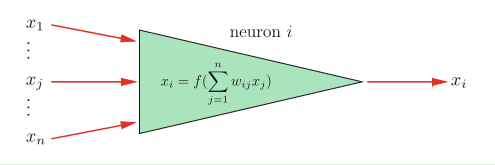
\includegraphics[width=8cm]{rys/neurony2.png}
		\caption{Struktura sztucznego neuronu, który stosuje funkcję skokową $f$ na ważonej sumie sygnałów wejściowych}
		\zrodlo{\cite{ertel}}
		\label{fig:neurony2}
	\end{figure}
\end{frame}

\begin{frame}{Warstwa gęsta}
	\begin{figure}[!h]
		\centering
		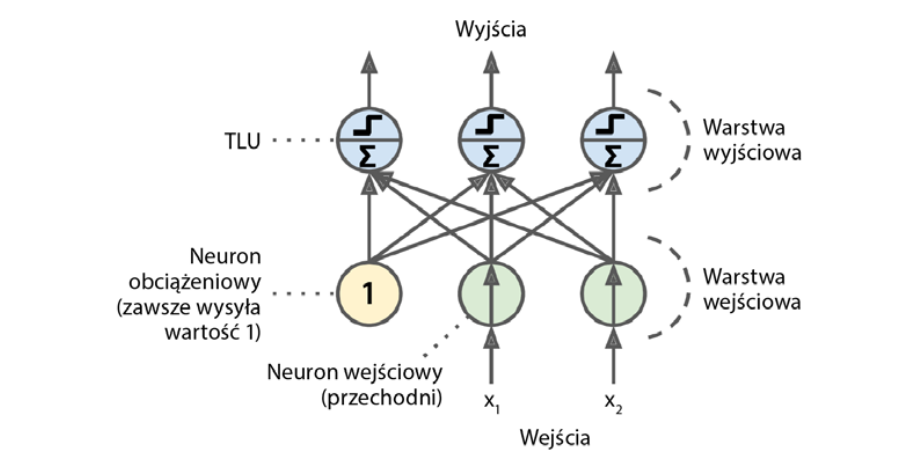
\includegraphics[width=\linewidth]{rys/perceptron1.png}
		\caption{Perceptron z trzema neuronami wejściowymi i trzema wyjściami}
		\zrodlo{\cite{geron}}
		\label{fig:perceptron1}
	\end{figure}
\end{frame}

\begin{frame}{Funkcje aktywacji}
	\begin{figure}[!h]
		\centering
		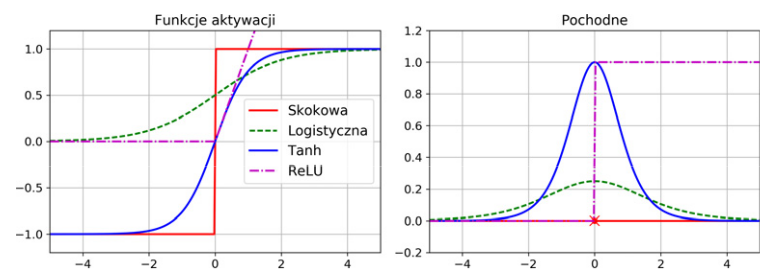
\includegraphics[width=\linewidth]{rys/funkcje_aktywacji.png}
		\caption{Przykładowe funkcje aktywacji wraz z pochodnymi}
		\zrodlo{\cite{geron}}
		\label{fig:funkcje-aktywacji}
	\end{figure}
\end{frame}
\subsection{Sieci splotowe}

\begin{frame}{Warstwa splotowa}
	\begin{figure}[!h]
		\centering
		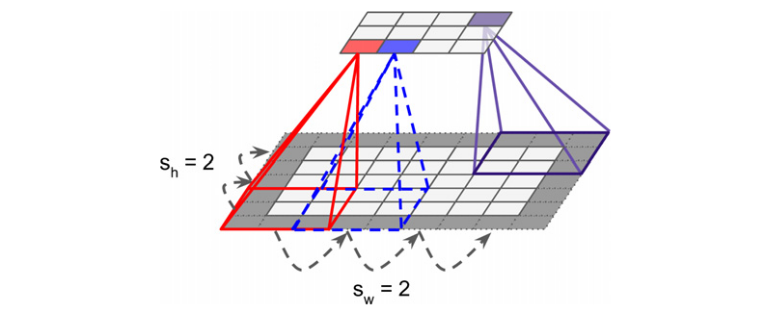
\includegraphics[width=0.9\linewidth]{rys/cnn_stride.png}
		\caption{Warstwa splotowa z krokiem o długości 2}
		\zrodlo{\cite{geron}}
		\label{fig:stride}
	\end{figure}
	
\end{frame}
\begin{frame}{Filtry i mapy cech}
	\begin{figure}[!h]
		\centering
		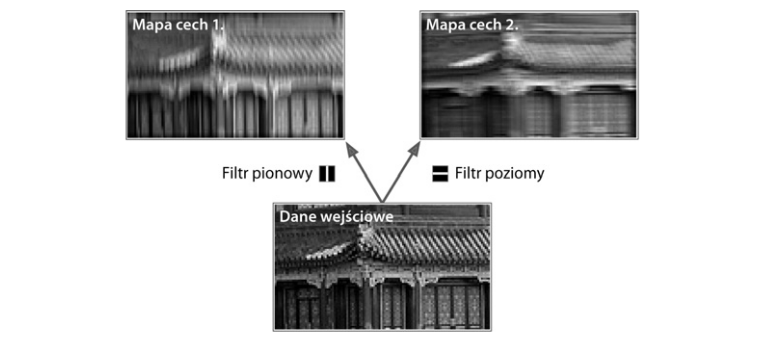
\includegraphics[width=0.9\linewidth]{rys/cnn_filtry.png}
		\caption{Uzyskiwanie dwóch map cech za pomocą dwóch różnych filtrów}
		\zrodlo{\cite{geron}}
		\label{fig:filtry}
	\end{figure}
\end{frame}

\begin{frame}{Warstwa łącząca}
	\begin{figure}[!h]
		\centering
		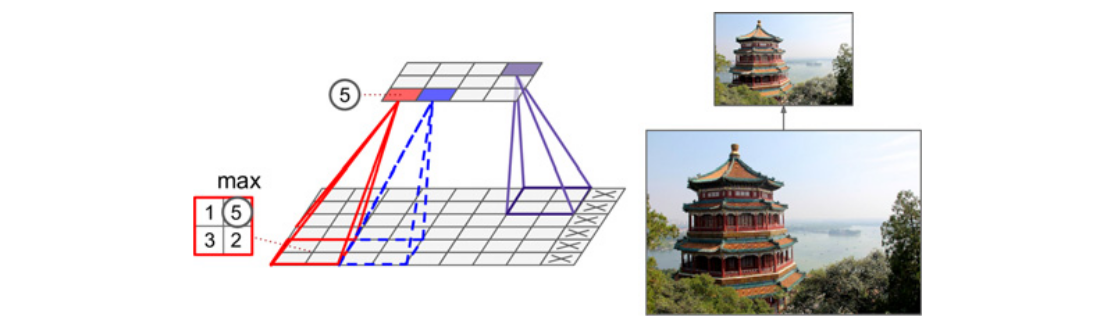
\includegraphics[width=\linewidth]{rys/max_pooling_layer.png}
		\caption{Maksymalizująca warstwa łącząca (jądro łączące: 2×2, krok: 2, brak uzupełniania zerami)}
		\zrodlo{\cite{geron}}
		\label{fig:max-pooling-layer}
	\end{figure}
\end{frame}
\begin{frame}{Warstwy ekspansji}
	\begin{figure}[!h]
		\centering
		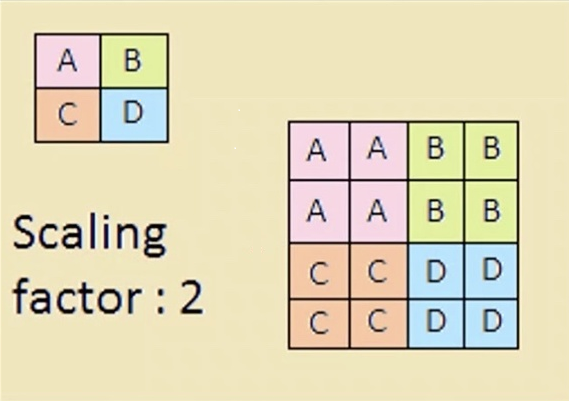
\includegraphics[width=0.7\linewidth]{rys/upsampling2d.png}
		\caption{Działanie warstwy ekspansji (nadpróbkowania)}
		\zrodlo{\cite{upsampling}}
		\label{fig:upsampling2d}
	\end{figure}
\end{frame}
\begin{frame}{Warstwy splotowe transponowane}
	\begin{figure}[!h]
		\centering
		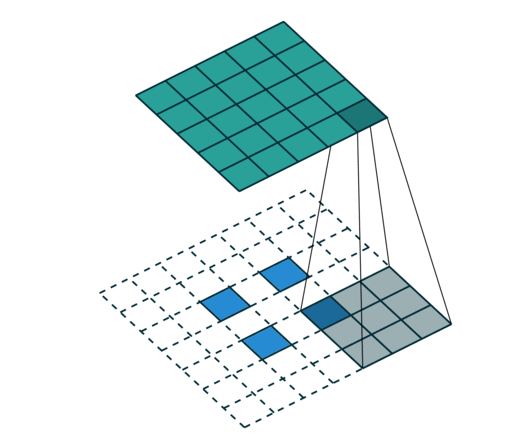
\includegraphics[width=0.6\linewidth]{rys/conv2dtranspose.png}
		\caption{Działanie warstwy splotowej transponowanej}
		\zrodlo{\cite{prove}}
		\label{fig:conv2dtranspose}
	\end{figure}
\end{frame}
\subsection{Autoenkodery}
\begin{frame}{Definicja autoenkodera}
	\begin{figure}[!h]
		\centering
		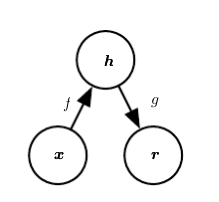
\includegraphics[width=5cm]{rys/autoencoder_structure.png}
		\caption{
			Struktura autoenkodera odwzorowującego wejście $x$ na wyjście $r$ (nazywane rekonstrukcją) poprzez reprezentację ukrytą (kodowanie) $h$. Autoenkoder składa się z dwóch składników: kodera $f$ (odwzorowującego $x$ na $h$) i dekodera $g$ (odwzorowującego $h$ na $r$)}
		\zrodlo{\cite{goodfellow}}
		\label{fig:autoencoder-structue}
	\end{figure}
\end{frame}
\begin{frame}{Rodzaje autoenkoderów}
	\begin{itemize}
		\item  autoenkodery niedopełnione (ang. \emph{undercomplete}), w których wyjście musi mieć mniejszy wymiar niż wejście
		\item autoenkodery z regularyzacją (ang. \emph{regularized}), w których wyjście ma taki sam lub większy (ang. \emph{overcomplete}) wymiar niż wyjście, ale używają specjalnie dopasowanych funkcji straty. Wśród autoenkoderów z regularyzacją można rozróżnić na przykład:
		\begin{itemize}
			\item autoenkodery rzadkie (ang. \emph{sparse}), które dążą do rzadkiej reprezentacji ukrytej
			\item autoenkodery odszumiające (ang. \emph{denoising}), które na wejściu dostają zniekształcone dane, a starają się odzyskać pierwotne, niezaszumione informacje
			\item autoenkodery kurczliwe (ang. \emph{contractive}) dążące do małego rozmiaru pochodnej
		\end{itemize}
	\end{itemize}
\end{frame}
\begin{frame}{Rodzaje autoenkoderów}
	\begin{itemize}
		\item autoenkodery stosowe (ang. \emph{stacked}) nazywane również głębokimi (ang. \emph{deep})
		\item autoenkodery splotowe (ang. \emph{convolutional})
		\item autoenkodery rekurencyjne (ang. \emph{recurrent})
		\item autoenkodery wariancyjne (ang. \emph{variational})
		\item autoenkodery przeciwstawne (ang. \emph{adversial})
	\end{itemize}
\end{frame}
\begin{frame}{Zastosowania autoenkoderów}
	\begin{enumerate}
		\item  Zmniejszenie wymiarowości (ang. \emph{Dimensionality Reduction })
		
		\item  Wyodrębnianie cech (ang. \emph{Feature Extraction})
		
		\item  Odszumianie obrazu (ang. \emph{Image Denoising })
		
		\item  Kompresja obrazu (ang. \emph{Image Compression})
		
		\item Wyszukiwanie obrazu (ang. \emph{ Image Search })
		
		\item Wykrywanie anomalii (ang. \emph{ Anomaly Detection})
		
		\item  Uzupełnianie brakujących danych (ang. \emph{Missing Value Imputation })
		
	\end{enumerate}
\end{frame}
\section{Zastosowania}
\subsection{Prosty autoenkoder}
\begin{frame}{Struktura prostego autoenkodera}
	\begin{figure}[!h]
	\centering
	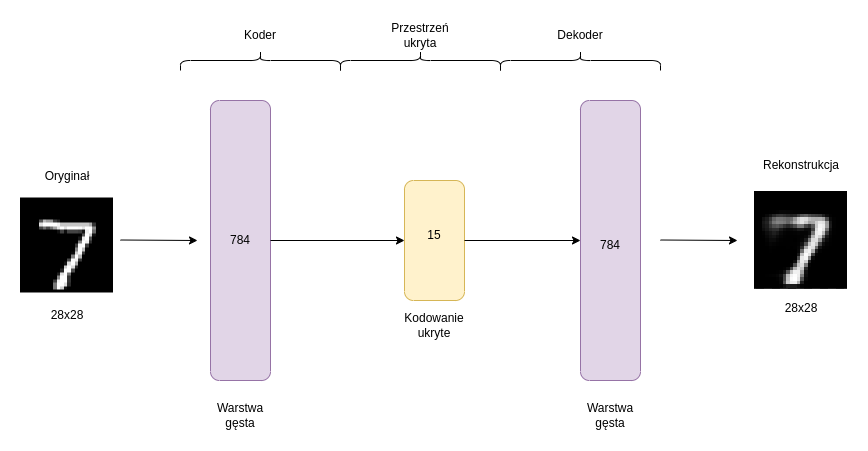
\includegraphics[width=0.9\linewidth]{diagramy/ae_simple.drawio.png}
	\caption{Struktura autoenkodera prostego (niedopełnionego)}
%	\label{fig:simple-encoded}
	\zrodlo{Opracowanie własne}
\end{figure}
	
\end{frame}

\begin{frame}{Reprezentacja ukryta i rekonstrukcje}
	\begin{figure}[!h]
		\centering
		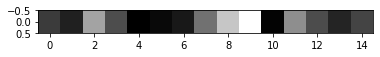
\includegraphics[width=0.6\linewidth]{rys2/simple_encoded.png}
		\caption{Reprezentacja 15-wymiarowa dla pierwszej obserwacji ze zbioru testowego MNIST}
		\label{fig:simple-encoded}
		\zrodlo{Opracowanie własne}
	\end{figure}

\begin{figure}[!h]
	\centering
	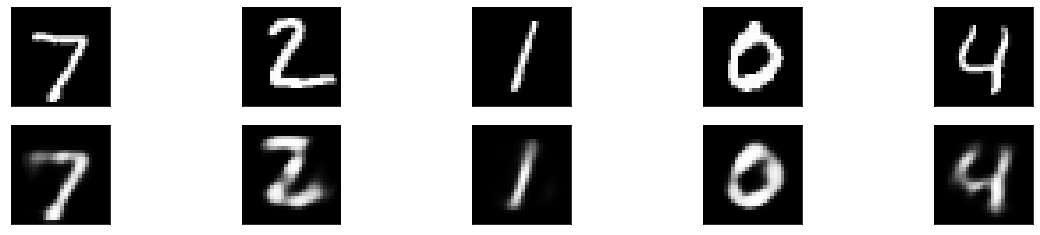
\includegraphics[width=\linewidth]{rys2/simple_reconstructions.png}
	\caption{Pięć pierwszych obserwacji ze zbioru testowego MNIST: w górnym rzędzie oryginalne obrazy, w dolnym rekonstrukcje z autoenkodera niedopełnionego}
	\label{fig:simple-reconstructions}
	\zrodlo{Opracowanie własne}
\end{figure}

\end{frame}

\subsection{Autoenkoder splotowy}
\begin{frame}{Struktura autoenkodera splotowego}

		\begin{figure}[!h]
		\centering
		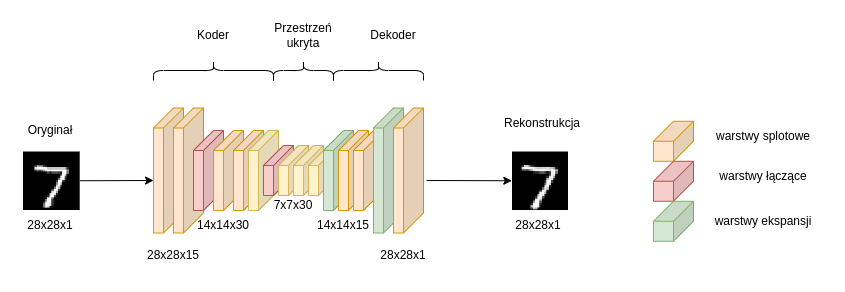
\includegraphics[width=\linewidth]{diagramy/ae_splotowy.drawio.png}
		\caption{Struktura autoenkodera splotowego}
		%	\label{fig:simple-encoded}
		\zrodlo{Opracowanie własne}
	\end{figure}

\end{frame}


\begin{frame}{Rekonstrukcje z autoenkodera splotowego}
	\begin{figure}[!h]
		\centering
		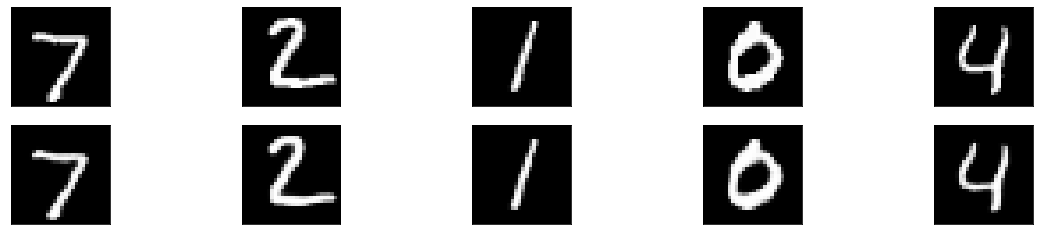
\includegraphics[width=\linewidth]{rys2/conv_reconstructions.png}
		\caption{Pięć pierwszych obserwacji ze zbioru testowego MNIST: w górnym rzędzie oryginalne obrazy, w dolnym rekonstrukcje z autoenkodera splotowego}
		\label{fig:conv-reconstructions}
		\zrodlo{Opracowanie własne}
	\end{figure}
	
\end{frame}

\begin{frame}{Porównanie funkcji strat z autoenkodera prostego i splotowego}
	\begin{figure}
			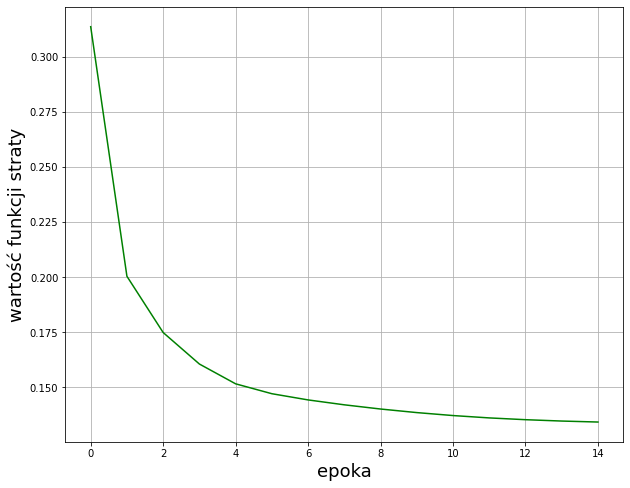
\includegraphics[width=0.475\linewidth]{rys2/simple_loss.png}
			\hfil
			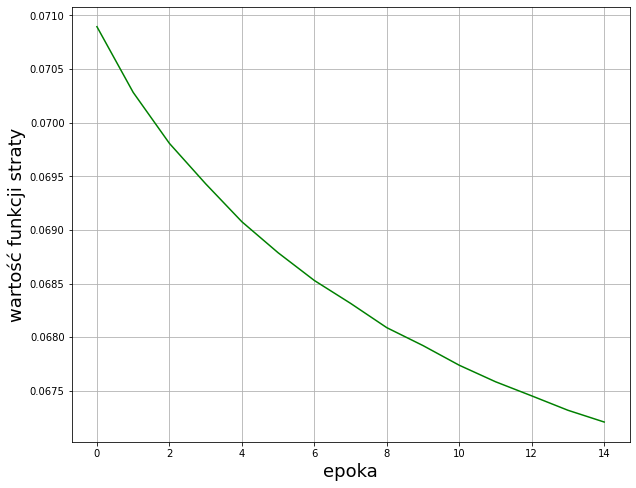
\includegraphics[width=0.475\linewidth]{rys2/conv_loss.png}
			\caption{Porównanie straty z autoenkodera prostego (po lewej) i splotowego (po prawej)}
			\zrodlo{Opracowanie własne}
	
	\end{figure}
\end{frame}
\subsection{Autoenkoder odszumiający}
\begin{frame}{Zaszumione obrazy}
	\begin{figure}[!h]
		\centering
		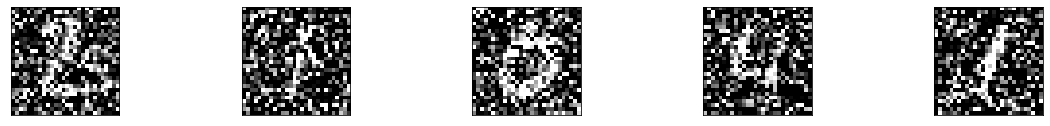
\includegraphics[width=\linewidth]{rys2/MNIST_noisy.png}
		\caption{Zaszumione obrazy ze zbioru testowego MNIST}
		\label{fig:MNIST-noisy}
		\zrodlo{Opracowanie własne}
	\end{figure}
\end{frame}

\begin{frame}{Struktura autoenkodera odszumiającego}
		\begin{figure}[!h]
		\centering
		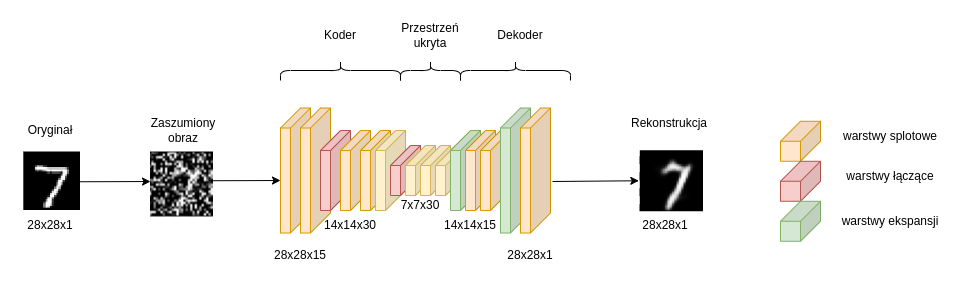
\includegraphics[width=\linewidth]{diagramy/ae_denoising.drawio.png}
		\caption{Struktura autoenkodera odszumiającego}
		%	\label{fig:simple-encoded}
		\zrodlo{Opracowanie własne}
	\end{figure}
	
\end{frame}


\begin{frame}{Odszumione rekonstrukcje}
	\begin{figure}[!h]
		\centering
		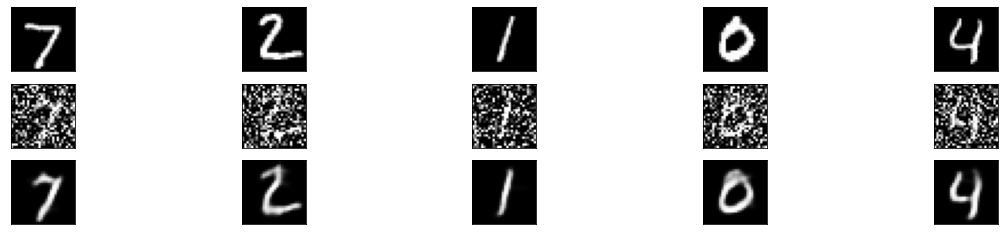
\includegraphics[width=\linewidth]{rys2/denoising_reconstructions.png}
		\caption{Pięć pierwszych obserwacji ze zbioru testowego MNIST: w górnym rzędzie oryginalne obrazy, w środkowym zaszumione, w dolnym rekonstrukcje z autoenkodera odszumiającego}
		\label{fig:denoising-reconstructions}
		\zrodlo{Opracowanie własne}
	\end{figure}
\end{frame}

\subsection{Wyszukiwanie obrazu}

\begin{frame}{Wyszukiwanie obrazu}
		\begin{figure}[!h]
		\centering
		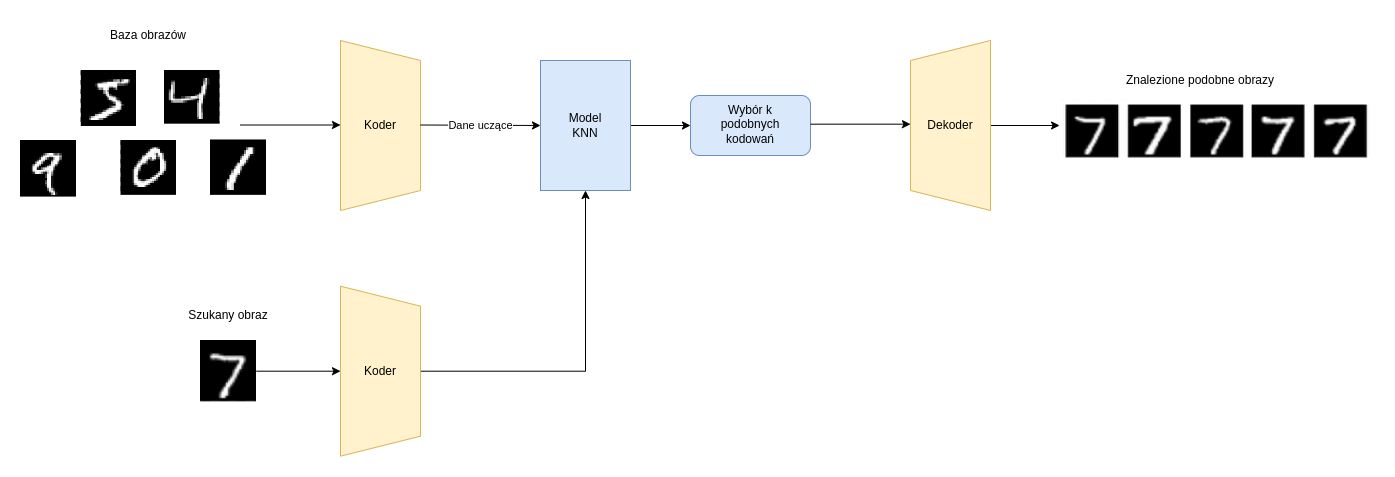
\includegraphics[width=\linewidth]{diagramy/image_retrieval.drawio.png}
		\caption{Schemat działania wyszukiwania obrazów przy użyciu autoenkodera}
		%	\label{fig:simple-encoded}
		\zrodlo{Opracowanie własne}
	\end{figure}
\end{frame}

\begin{frame}{Wyszukiwanie obrazu}
	\begin{figure}[!h]
		\centering
		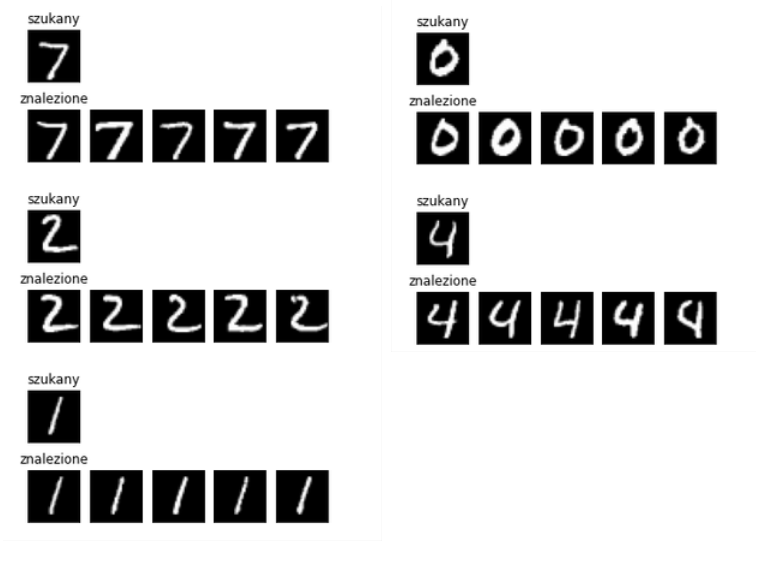
\includegraphics[width=0.7\linewidth]{rys2/retrieval_results_2cols.png}
		\caption{Wyniki zastosowania prostego autoenkodera przy wyszukiwaniu obrazu}
		\label{fig:retrieval-results}
		\zrodlo{Opracowanie własne}
	\end{figure}
\end{frame}

\subsection{Wykrywanie anomalii}

\begin{frame}{Struktura autoenkodera użytego do wykrywania anomalii}
	\begin{figure}[!h]
	\centering
	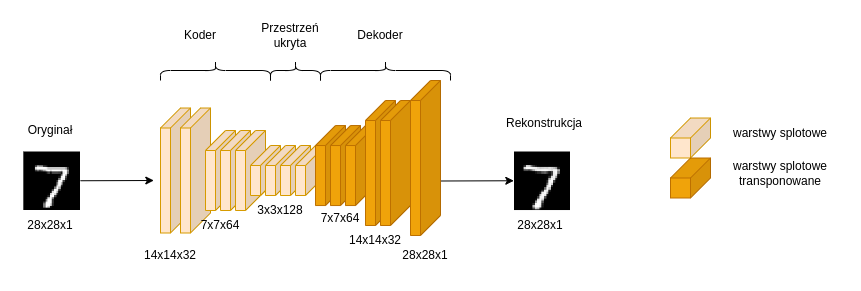
\includegraphics[width=0.9\linewidth]{diagramy/ae_anomalie.drawio.png}
	\caption{Struktura autoenkodera splotowego użytego do wykrywania anomalii}
	%	\label{fig:simple-encoded}
	\zrodlo{Opracowanie własne}
\end{figure}
\end{frame}

\begin{frame}{Wykrywanie anomalii}
		\begin{figure}[!h]
		\centering
		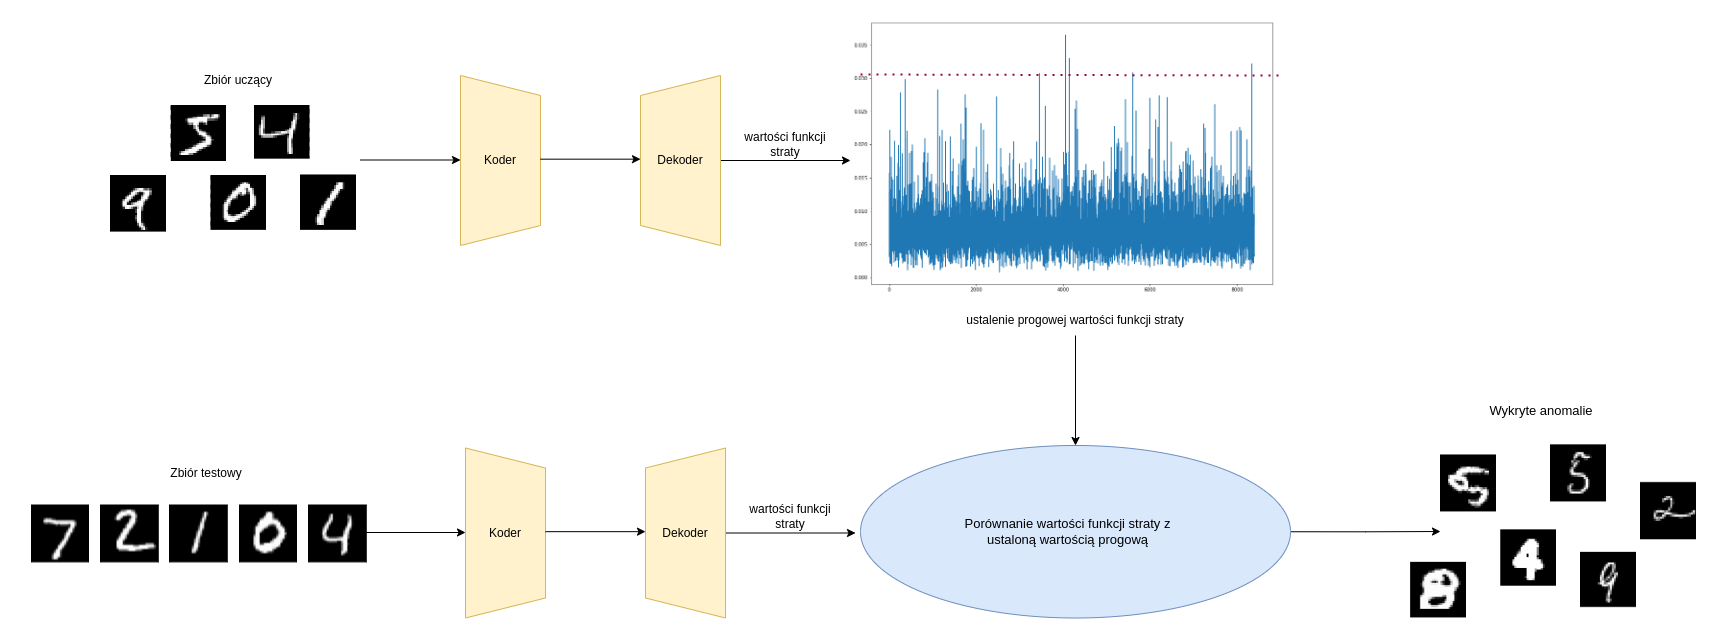
\includegraphics[width=\linewidth]{diagramy/anomaly_detection.drawio.png}
		\caption{Schemat wykrywania anomalii przy użyciu autoenkodera}
		%	\label{fig:simple-encoded}
		\zrodlo{Opracowanie własne}
	\end{figure}
\end{frame}

\begin{frame}{Graniczna wartość straty}
		\begin{figure}[!h]
		\centering
		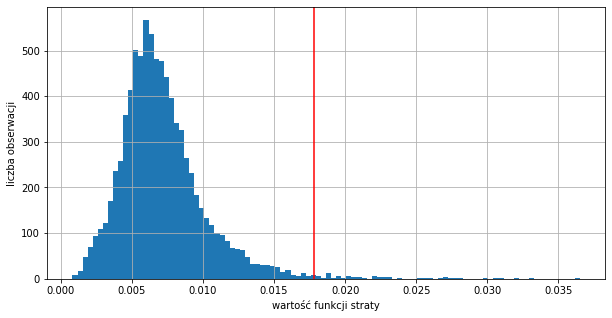
\includegraphics[width=0.7\linewidth]{rys2/anomaly_loss_threshold.png}
		\caption{Histogram funkcji straty}
		\label{fig:ae-wykryte-anomalie}
		\zrodlo{Opracowanie własne}
	\end{figure}
\end{frame}

\begin{frame}{Przykłady wykrytych anomalii}
	\begin{figure}[!h]
		\centering
		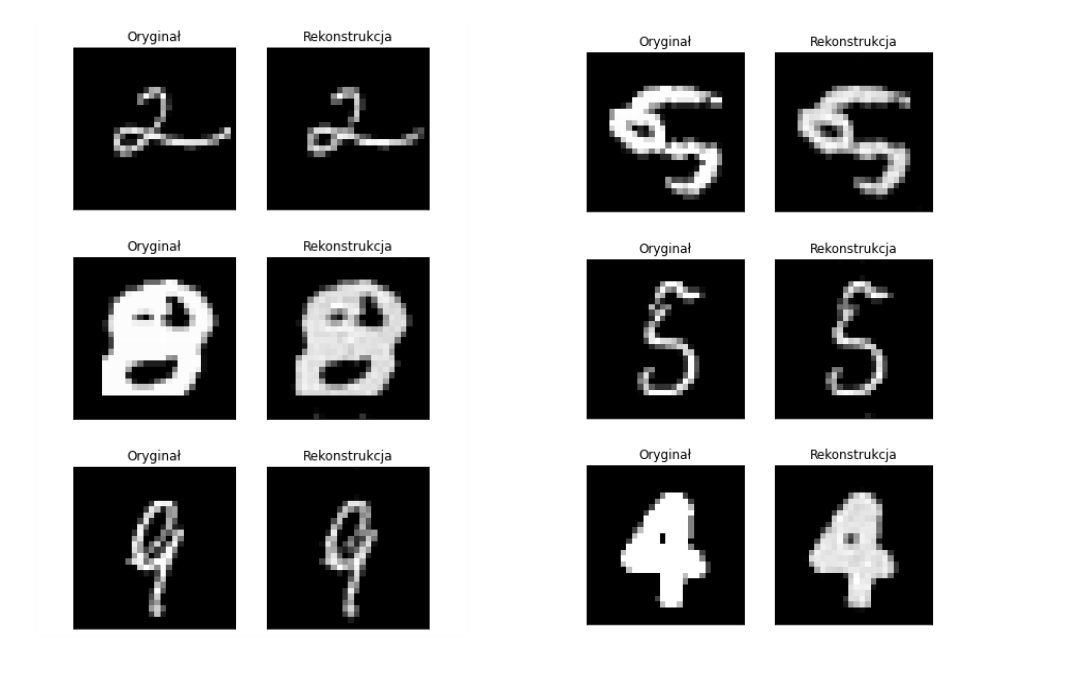
\includegraphics[width=0.7\linewidth]{rys2/ae_wykryte_anomalie.png}
		\caption{Przykłady anomalii w zbiorze MNIST wykrytych za pomocą autoenkodera}
		\label{fig:ae-wykryte-anomalie}
		\zrodlo{Opracowanie własne}
	\end{figure}
\end{frame}

\subsection{Generowanie obrazów}
\begin{frame}{Struktura autoenkodera wariancyjnego}
	\begin{figure}[!h]
	\centering
	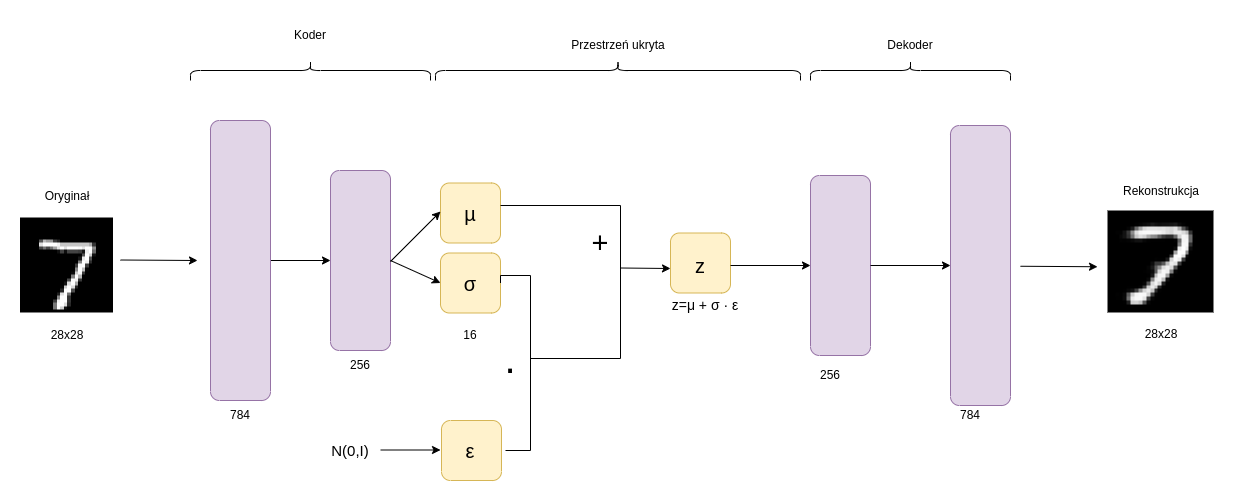
\includegraphics[width=\linewidth]{diagramy/ae_wariancyjny.drawio.png}
	\caption{Struktura autoenkodera wariancyjnego}
	%	\label{fig:simple-encoded}
	\zrodlo{Opracowanie własne}
\end{figure}
\end{frame}

\begin{frame}{Przestrzeń ukryta autoenkodera wariancyjnego}
	\begin{figure}[!h]
		\centering
		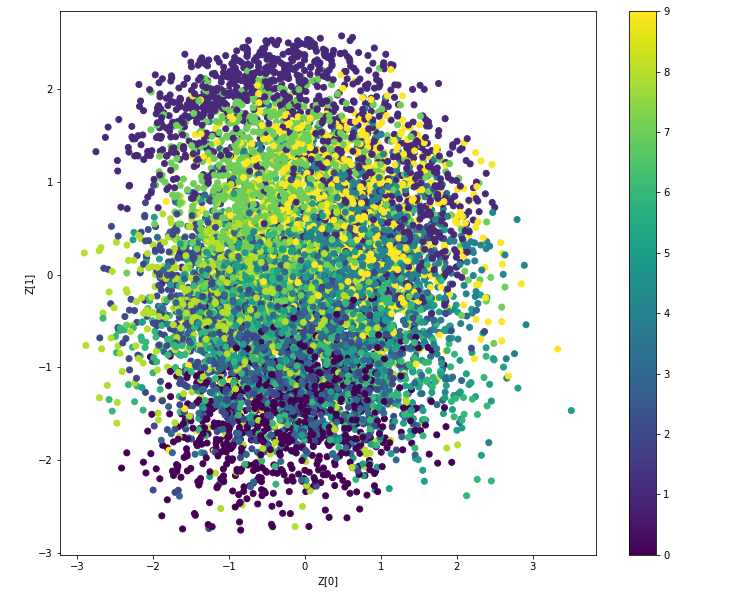
\includegraphics[width=0.6\linewidth]{rys2/latent_space_MNIST.png}
		\caption{Przestrzeń ukryta autoenkodera wariancyjnego}
		\label{fig:vae-latent-space}
		\zrodlo{Opracowanie własne}
	\end{figure}
\end{frame}

\begin{frame}{Przykłady wygenerowanych obrazów}
	\begin{figure}[!h]
		\centering
		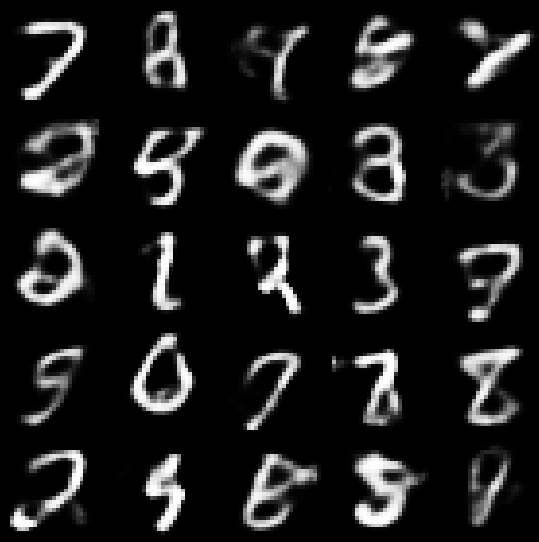
\includegraphics[width=0.5\linewidth]{rys2/vae_generated.png}
		\caption{Przykłady obrazów cyfr wygenerowanych przez autoenkoder wariancyjny}
		\label{fig:vae-generated}
		\zrodlo{Opracowanie własne}
	\end{figure}
\end{frame}
\begin{frame}{Autoenkoder wariancyjny}
\begin{figure}[!h]
	\centering
	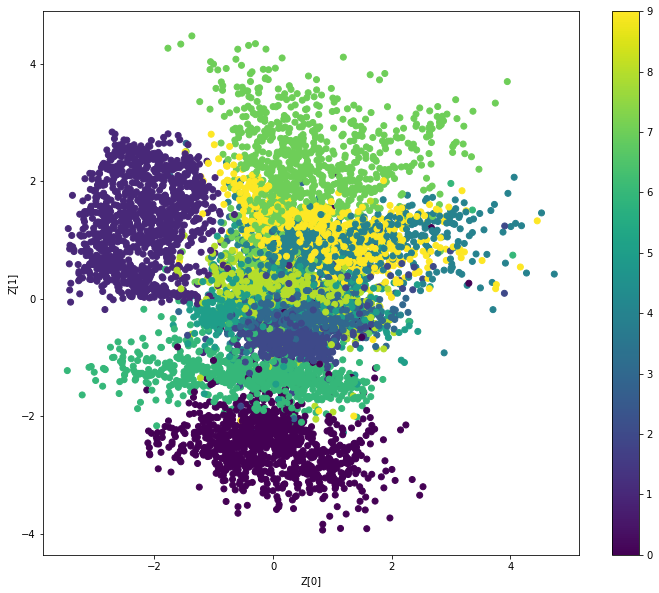
\includegraphics[width=0.5\linewidth]{rys2/latent_space_2dims.png}
	\caption{Przestrzeń ukryta autoenkodera wariancyjnego z wymiarem kodowania ukrytego równym dwa}
	\label{fig:vae-latent-space-2dims}
	\zrodlo{Opracowanie własne}
\end{figure}
\end{frame}

\begin{frame}{Autoenkoder wariancyjny}
\begin{figure}[!h]
	\centering
	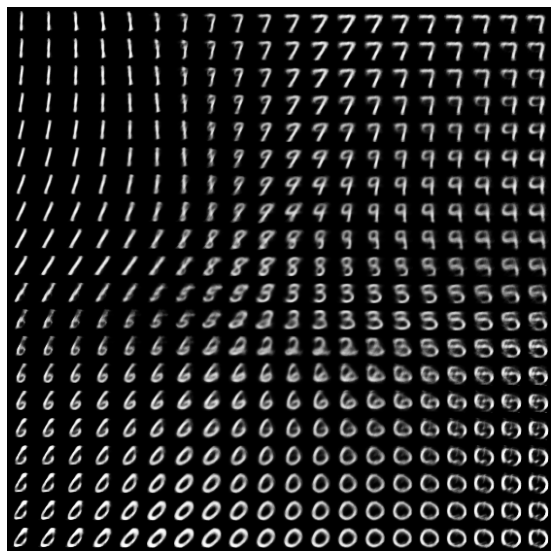
\includegraphics[width=0.5\linewidth]{rys2/latent_generated_2dims.png}
	\caption{Przestrzeń ukryta w postaci obrazów cyfr}
	\label{fig:vae-latent-generated-2dims}
	\zrodlo{Opracowanie własne}
\end{figure}
\end{frame}

\section{Bibliografia}

\begin{thebibliography}{99}
	
	\bibitem{upsampling} Artificial Intelligence in Plain English, \emph{Convolutional Autoencoders (CAE) with Tensorflow} \url{https://ai.plainenglish.io/convolutional-autoencoders-cae-with-tensorflow-97e8d8859cbe} (dostęp: 15.05.2022)
	
	\bibitem{ertel} Ertel W. (2017) \emph{Introduction to Artificial Intelligence. Second Edition}, Springer International Publishing
	\bibitem{geron} G\'eron A. (2020) \emph{Uczenie maszynowe z użyciem Scikit-Learn i TensorFlow. Wydanie II}, Helion SA
	\bibitem{goodfellow} Goodfellow I., Bengio Y., Courville A. (2018), \emph{Deep Learning. Systemy uczące się}, PWN, Warszawa 
	
	\bibitem{prove} Pröve P. L., \emph{An Introduction to different Types of Convolutions in Deep Learning}, \url{https://towardsdatascience.com/types-of-convolutions-in-deep-learning-717013397f4d} (dostęp: 15.05.2022)
	
	
\end{thebibliography}

\end{document}